

% System Architecture

% Data - user document matrix, item document matrix, user-item matrix


% chatbot system - talking to user
% -- using nlp to extract topic / feature (e.g. actor, film genre)
% -- using nlp to extract sentiment


% -- using nlp to generate responses
% -- using LLM's guide user to explore preferences

% Explainability - system has to be able to explain why it made a recommendation and how it came to that conclusion
% -- explain users current preferences
% -- explain why a recommendation was made


% weighting scheme system

% recommendation system - recommending items to user
% -- using user-item matrix to recommend items
% -- using item document matrix to provide information on items
% -- using nlp to generate item descriptions

% use both explicit feedback from chats and implicit feedback from user-item matrix to improve recommendations
% hybrid system - combining collaborative and content-based filtering + explicit NLP chat feedback


% ---- break ---- seperate part
%

% evaluation system - evaluating the system
% -- using user-item matrix to evaluate recommendations
% -- using user document matrix to evaluate user preferences
% -- using nlp to evaluate user responses


\begin{figure}
    \centering
    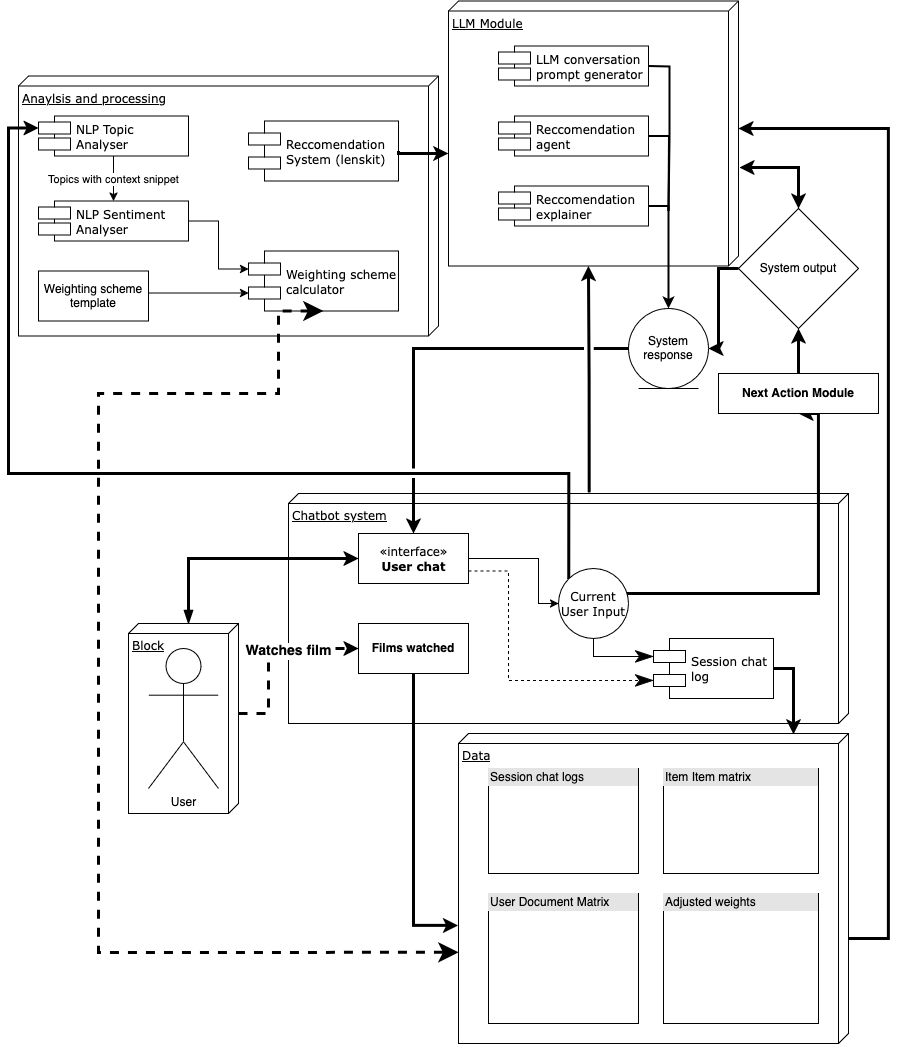
\includegraphics[width=0.8\textwidth]{Figures/FYP_HLA.drawio.png}
    \caption{WIP: System HLA}
    \label{fig:systemHLA}
\end{figure}

\subsection{System Architecture}
\label{sec:systemArchitecture}
The system will be built with a multi-agent approach, with each agent responsible for a different aspect of the system.

I will be building the project in steps, where I am keeping each component as modular as possible to allow for easy integration and testing.

The system will be built with the following components:
\begin{itemize}
    \item \textbf{Chat interface}: The user interface for the user to interact and converse with the system.
    \item \textbf{NLP System}
    \subitem \textbf{Topic Extraction}: Extracting topics and features from the user's messages.
    \subitem \textbf{Sentiment Analysis}: Extracting topic sentiment from the user's messages.

    \item \textbf{Reccomendation System}:
    \subitem \textbf{Recommendation Generation}: Generating recommendations for the user.
    \subitem \textbf{Recommendation Explaination Metrics}: Outputs the key metrics used to generate the recommendation.

    \item \textbf{LLM Module}: Using Large Language Models to converse with the user.
    \subitem \textbf{User Preference Exploration}: Using LLMs to guide the user to explore their preferences.
    \subitem \textbf{Recommendation Explainability}: Using LLMs to explain why a recommendation was made taking in reccomendation explaination metrics.


    \item \textbf{Weighting Scheme System}: This component will be responsible for weighting the user's preferences and the system's recommendations.
    \item \subitem \textbf{User Preference Weighting}: Adjusts the users weighting scheme by takign NLP sentiment analysis into account.
    \item \subitem \textbf{Recommendation Weighting}: Weights the system's recommendations.

\end{itemize}






